\textbf{
\begin{center}
ОБЩАЯ ХАРАКТЕРИСТИКА РАБОТЫ
\end{center}
}
\textbf{Актуальность исследования.}
\emph{Автоматизация антропометрических измерений} -- важная область приложения методов компьютерного зрения в математическом моделировании\footnote{Шапиро, Л. Компьютерное зрение = Computer Vision : [учеб. пособие] / Дж. Стокман, ред.: С. М. Соколов, пер.: А. А. Богуславский, Л. Шапиро .— 2-е изд. (эл.) .— М. : БИНОМ. Лаборатория знаний., 2013 .— 762 с.}. Задача антропометрии состоит в обнаружении человеческого тела на изображении, распознавании его частей (головы, рук, ног и т.п.), описании антропометических признаков (размеров частей тела) с целью создания соответствующей 3D-модели\footnote{Грудинин, С.Н. Предметная параметризация виртуальных манекенов [Текст] / С.Н. Грудинин, В.Д. Фроловский // Автоматика и программная инженерия.- 2014. – № 1 (7). – С. 53–56.}. В здравоохранении (измерение размеров тела, фитнес-тестирование), проектировании и пошиве одежды, обеспечении безопасности и разработке систем мониторинга движения (X. Yan 2014), локализации и распознавании деятельности человека на изображении (M. Jainy 2015) требуется решение задач антропометрии с заданной точностью и скоростью (A. Konstantinos 2016). Этим проблемам посвящен ряд современных исследований. Например, в работе (YuChen 2011) предложена модель, позволяющая обнаруживать человека на статических изображениях. Barron и Kakadiaris (C. Barron 2000) и Taylors (C.J. Taylor 2000) создали алгоритмы восстановления 3D-модели человеческого тела. В работах (A.S. Micilotta 2005) рассмотрена задача распознавания основных частей тела. На практике используются различные способы регистрации изображений, допускающие искажения и шум во входных данных, которые восстанавливаются при помощи большого арсенала современных методов\footnote{Ярославский, Л.П. Введение в цифровую обработку изображений [Текст] / Л.П. Ярославский //– М.: Сов. радио, 1979. – 312 с.}\footnote{Белявцев, В.Г., Воскобойников, Ю.Е. Алгоритмы фильтрации изображений с адаптацией размеров апертуры [Текст] / В.Г. Белявцев, Ю.Е. Воскобойников // Автометрия. – 1998. – № 3. – С. 18 – 25.}\footnote{Сизиков, В.С. Обратные прикладные задачи и MatLab [Текст] / В.С. Сизиков. - Санкт-Петербург : СПб: Лань, 2011. - С.256 с.}\footnote{Kokaram, A.C. Motion Picture Restoration: Digital Algorithms for Artefact Suppression in Degraded Motion Picture Film and Video [Text] / A.C. Kokaram //Springer Science \& Business Media, 2013. -334 p.}\footnote{Sidorov, D. Integral Dynamical Models: Singularities, Signals \& Control [Text] / D. Sidorov. - Singapore: World Scientific, 2015.}.

Дополнительным стимулом к развитию методов компьютерного зрения в антропометрии служит высокая популярность мобильных вычислительных устройств (смартфонов). Большой объем цифрового контента стимулирует создание новых методов интеллектуального анализа данных, обработки и анализа изображений и видео при ограниченных по сравнению с компьютерами общего назначения вычислительных ресурсах.

Таким образом, разработка новых эффективных методов бесконтактной экспресс-антропометрии является актуальной проблемой и представляет интерес для решения широкого спектра задач, возникающих в медицине, биометрии, фитнесе и моделировании одежды. Наконец, в последнее время приобретает большую популярность интернет-торговля и в этой области экспресс-антропометрия имеет большие перспективы как из-за отсутствия унифицированной системы размеров, так и в силу необходимости классификации типов телосложения.

Результаты данной работы представляют собой алгоритмическое обеспечение и программные технологии для решения некоторых из перечисленных выше задач антропометрии. А именно, диссертация посвящена актуальным проблемам развития средств математического моделирования, численных методов, алгоритмов и программного обеспечения для обработки изображений и видеопоследовательностей в задачах антропометрии. Разработанные программные модули обеспечивают необходимый уровень точности измерений параметров человеческого тела, позволяющих, в частности, строить практически значимые 3D-модели человеческого тела, а также позволяют решать поставленные задачи над входными данными, имеющими шумы, в режиме функционирования, близком к реальному времени, при этом в определенной степени снимаются ограничения вычислительных ресурсов мобильных устройств.

\textbf{Целью исследования} является совершенствование математических моделей, численных методов, алгоритмов компьютерного зрения, а также их реализация в виде комплекса программ антропометрии для мобильных вычислительных платформ. Для достижения указанной цели решены следующие \textbf {основные задачи}:
\begin{enumerate}
	\item[1)] Разработка алгоритмов и методов компьютерного зрения для извлечения антропометрических признаков из изображений и видеопоследовательностей в режиме, близком к реальному времени и при наличии шума;
	\item[2)] Создание гибридных методов и алгоритмов компьютерного зрения, позволяющих повысить производительность вычислений и точность извлечения антропометрических признаков\cEA{Тут будет вопрос о сравнении...};
	\item[3)] Применение методов машинного обучения для классификации данных антропометрических признаков\cEA{Лучше говорить о совершенствовании методов или разработке методики применения КЛАССА методов машинного для задачи антропометрии.};
	\item[4)] Создание методики построения 3D-моделей телосложения людей на основе полученных данных антропометрии. \mrk{Способ требует правильное описание структуры и формы человека с учетом полученных измерений\cEA{Это требование чего-то ко входным данным? или это свойства выходных данных?}};
	\item[5)] Разработка антропометических приложений для смартфонов с операционной системой Андроид для использования в моделировании одежды и в фитнес-тестировании. Оценка качества и эффективности функционирования полученной антропометрической системы.
\end{enumerate}
Результаты проведенных экспериментов подтвердили эффективность алгоритмов компьютерного зрения в антропометрии. Сравнение с результатами аналогичных исследований подтвердило эффективность\cEA{По какому критерию?} предложенных математических моделей и комплекса программ.

\textbf{Объект исследования} - методы и алгоритмы компьютерного зрения.

\textbf{Предмет исследования} - математическая модель, задачи, методики, алгоритмы и программы применительно к задаче антропометрии. Предмет исследования определен предметной областью №7 паспорта специальности 05.13.18 «Разработка новых математических методов и алгоритмов интерпретации натурного эксперимента на основе его математической модели», а так же перечнем задач решаемых в диссертации.

\textbf{Методы исследования.} Методы теоретических исследований: алгоритмы и методы компьютерного зрения в антропометрии; методы анализа данных и построения антропометрических моделей. Методы прикладных исследований: проектирование алгоритмов для задачи извлечения признаков и классификации антропометрических признаков; разработка 3D моделей для моделирования формы человеческого тела; разработка мобильных приложений; тестирование программ и хранение результатов, оценка и сравнение результатов.

\textbf{Научная новизна} результатов диссертационной работы заключается в следующем:

\begin{enumerate}
	\item[1)] Предложены методы математического моделирования различных типов телосложения на основе интеллектуального анализа антропометрических признаков, полученных с использованием алгоритмов компьютерного зрения;
	\item[2)] Адаптированы численные методы машинного обучения на основе случайного леса для классификации антропометрических измерений\cEA{Не понял, что такое ``классификация измерений''.};
	\item[3)] Разработаны методы визуализации моделей человеческого тела на основе антропометрических признаков, полученных при помощи авторских методов компьютерного зрения;
	\item[4)] Разработана бесконтактная система антропометрии для смартфона на операционной системе Андроид.
\end{enumerate}

\textbf{Практическая значимость и внедрение работы.} На основе предложенных моделей, методик и алгоритмов создано несколько приложений ОС Андроид для осуществления замеров одежды и параметров тела в медицине. Результаты исследования применены на практике при моделировании форменного обмундирования, получен акт о внедрении\cEA{Внедрение в фитнесе??}.

\textbf{Апробация работы.} Работа выполнена на кафедре вычислительной техники ИРНИТУ. Результаты диссертационной работы обсуждались и докладывались на симпозиумах, семинарах и конференциях: Всероссийские молодежные научно-практические конференции «Винеровские чтения» (Иркутск, 2014, 2015, ИРНИТУ); XIX Байкальская всероссийская конференция «Информационные и математические технологии в науке и управлении» (Улан-Удэ, 2014); The 4th, 5th International Conference on Analysis of Images, Social Networks, and Texts (Екатеринбург, 2015, 2016); V Научно-практическая Internet-конференция «Междисциплинарные исследования в области математического моделирования и информатики» (Тольятти, 2015). Работа выполнена при поддержке Министерства образования и подготовки кадров Социалистической Республики Вьетнам и программы развития ФГБУ ВО ИРНИТУ.

\textbf{Личный вклад автора.} Основные результаты выносимые на защиту получены автором лично. Конфликта интересов с соавторами нет.

\textbf{Публикации.} По теме диссертации опубликовано 11 научных работ, 4 из которых – в рецензируемых научных журналах и изданиях, рекомендованных ВАК РФ, 2 свидетельства регистрации программы на ЭВМ, одна статья опубликована в журнале, индексируемым Web of Science и одна статья опубликована в журнале, индексируемым Scopus.

\textbf{Структура и объем работы.} Диссертация содержит введение, четыре главы, заключение и список использованной литературы, содержащий 172 наименований. Общий объем диссертации составляет 130 страниц машинописного текста, иллюстрированного 58 рисунками и 5 таблицами.
%%%%%%%%%%%%%%%%%%%%%%%%%%%%%%%%%%%%%%%%%%%%%%%%%%%%%%%%%%%%%%%%%%%
\begin{center}
\textbf{ОСНОВНОЕ СОДЕРЖАНИЕ РАБОТЫ}
\end{center}

Во \textbf{введении} обосновывается актуальность исследований, на основании чего сформулированы цель и задачи работы; определены объект, предмет, методы и средства исследования; раскрыта научная новизна и практическая значимость полученных результатов; изложены основные научные положения, выносимые на защиту; приведены структура и краткий обзор содержания работы.

В \textbf {первой главе} анализируются алгоритмический подход и методы компьютерного зрения в извлечении антропометрических признаков\footnote{3635-99, ГОСТ Р ИСО. Одежда. Размеры. Определения, обозначения и требования к измерению [Электронный ресурс] // [http://www.internet-law.ru/gosts/gost/8932]. -- [Б. м. : б. и.]. -- Дата доступа: 2017.}\footnote{13402, EN. Европейский стандарт указания размеров одежды [Электронный ресурс] // [https://ru.wikipedia.org/wiki/EN-13402] -- [Б. м. : б. и.]. -- Дата доступа: 2017.} со статических изображений и видеопоследовательностей. Излагаются алгоритмы построения опорных точек из видеопоследовательностей, рассматриваются принципы формирования 3D моделей на основе сопоставления опорных точек человеческого тела в построенных моделях.

На основе проведенного анализа\cEA{Литературы? или еще какой-то анализ осуществлялся?} сделан вывод об адекватности и точности использования комбинированных методов и соответствующих алгоритмов -- итеративного алгоритма ближайших точек (ИАБТ), разрезов на графах -- для извлечения антропометрических признаков, при использовании метода случайного леса (Random Forest) для классификации антропометрических данных в статических изображениях и видео в присутствии шума, в режиме близком к реальному времени. Такой подход позволил построить систему компьютерного зрения в антропометрии обладающую с высокой точностью и скоростью обработки.

\textbf{Вторая глава} посвящена построению математической модели и численных методов компьютерного зрения к задаче антропометрии. \mrk{В этой главе решаются следующие задачи:}
\begin{itemize}
	\item разработка математических моделей и численных методов компьютерного зрения для извлечения антропометрических признаков;
	\item приложение математических моделей и численных методов машинного обучения для классификации антропометрических данных;
	\item разработка метода построения антропометрических моделей.\cEA{Это уже 2 раза ВСЕ было.}
\end{itemize}

В \textbf{п.~2.1} для решения задачи извлечения антропометрических признаков из изображений и видеопоследовательностей (см. рис.\ref{img53}) предложен алгоритм, основанный на комбинации  методов предварительной обработки изображений (\cEA{Что за метод?}), алгоритме вычитания фона, алгоритме сегментации изображений на основе разреза на графах и итеративного алгоритма ближайших точек.
\begin{figure}[ht!]
\centering
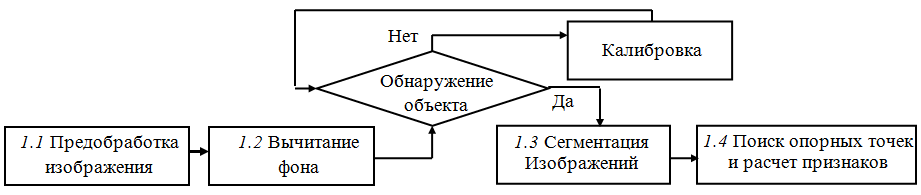
\includegraphics [width=1\linewidth] {images/h53.png}
\begin{center}
%\captionsetup{justification=justified, labelsep=period}
\caption{Блок-схема процесса извлечения антропометрических признаков.} \label{img53}
\end{center}
\end{figure}

На этапе предварительной обработки изображения (\textbf{п.2.2.1}) происходит преобразование входного изображения из формата RGB в полутоновое изображение, подавляется шум, выполняется сглаживание изображения, проводится эквализация гистограммы, применяются морфологические операторы для улучшения качества контура объекта.

На этапе обнаружения объектов (\textbf{п.2.2.2}) выполняется вычитание фона (C. Stauffer 1999). Результатом является область изображения, которая содержит человеческое тело (область интереса - ROI). К извлеченной области далее будет применена сегментация. Отбор пикселей, принадлежащих фону и объекту проводится с использованием бинарного изображения (маски). Считается, что пиксель принадлежит объекту и имеет белый цвет в маске, если разность интенсивности фона и текущего кадра для данного пикселя превышает некоторое пороговое значение.

\textit{1.3 Сегментация изображений на основе метода разрезов на графах (Y. Boykov 2004) (п.2.2.3).}

\begin{figure}[ht!]
\centering
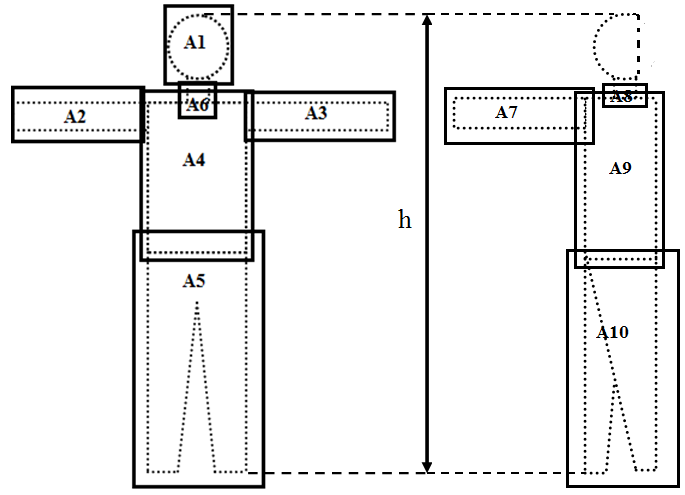
\includegraphics [width=0.45\linewidth] {images/h111.png}
\begin{center}
%\captionsetup{justification=justified, labelsep=period}
\caption{Моделирование телосложения для сегментации изображения. h (рост) - параметр калибровки.} \label{img1}
\end{center}
\end{figure}
Предположим, что множество $S=\left\{s_i|i=1, ..., n\right\}$ представляет собой область интереса, которую получили после вычитания фона.
Сегментация определяется набором случайной величины $A=\left\{A_i|i=1, ..., n\right\}$, $A_i\in L $ которого указывает маркировка $s_i$ и $L=\left\{L_j|j=1, ..., m\right\}$ является набором меток.

Каждый ROI имеет области, которые содержит части человеческого тела: голова, шея, руки, ноги и тело. Проводится калибровка с учетом параметров камеры и параметра h (см. рис. \ref{img1}). Одним из эффективных методов сегментации является метод минимального разреза - максимального потока. В этом случае алгоритм трактует всё изображение как граф $G\left(V, E\right)$. Элементы множества $V$ называются вершинами-пикселями графа, а пары из $E$ — его рёбрами. В полученном графе находится минимальный разрез, который делит граф на 2 части. Пиксели, попавшие в один подграф с истоком, считаются областями частей человеческого тела, остальные пиксели признаются областями где нет частей человеческого тела. Результаты сегментации используются далее на этапе обработки и анализа контура каждой части человеческого тела.

\textit{1.4 Построение опорных точек на основе итеративного алгоритма ближайших точек (ИАБТ) (Z. Zhang 1992) (п.2.2.4).} Пусть $A=\left\{a_i| i=1, ..., n\right\}$ представляет собой набор точек контура частей человеческого тела. $B=\left\{b_i| i=1, ..., m\right\}$ является модельным набором координат для обнаружения искомых опорных точек. Цель алгоритма ИАБТ состоит в поиске набора точек доставляющих минимум расстояния между наборами А и B:

\begin{algorithm}[ht!]
  \KwData{2 облака точек $A=\left\{a_i\right\}$, $B=\left\{b_i\right\}$; начальное преобразование $T_0$}
  \KwResult{итоговое преобразование $T$ для обнаружения опорных точек в $A$,}
  $T\leftarrow T_0$\;
  \While{\texttt{не сходится}}{
	\For{\texttt{$i\leftarrow 1$ to $n$}}
     {
		$m_i \leftarrow$ Найти ближайшие точки в $A$ к $T\ast b_i$;

		\eIf{$\left\|m_i -T\ast b_i\right\|\leq d_{max}$}{
      $w_i \leftarrow 1$;
    }{
       $w_i \leftarrow 0$;
    }
   }
	$T\leftarrow argmin_{T}\left\{\sum_i w_i\left\|T\ast b_i -m_i\right\|^2\right\}$;\\
	$n=n+1$;
		}
  \caption{Описание алгоритма ИАБТ}
\end{algorithm}

Поиск итогового расположения опорных точек на найденных опорных контурах для каждой ROI (рис. \ref{img1}) осуществляется согласно ГОСТ$^4$. Результаты обнаружения опорных точек представлены на рис. \ref{img7}.
\begin{figure}[ht!]
\centering
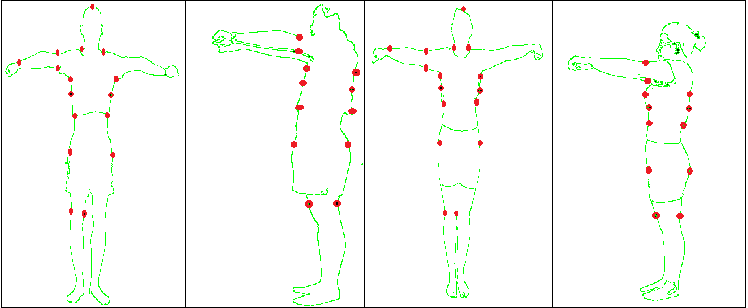
\includegraphics [width=0.9\linewidth] {images/h18.png}
\begin{center}
%\captionsetup{justification=justified, labelsep=period}
\caption{Результаты обнаружения опорных точек.} \label{img7}
\end{center}
\end{figure}
Расчеты проводятся с использованием евклидова расстояния. С такими антропометрическими признаками, как длина руки, длина плеча и т.д. (несложная геометрия) использовалось непосредственно евклидово расстояние между соответствующими опорными точками. Для извлечения антропометрических признаков со сложной структурой (талия, грудь, бедро) необходимо было использовать больше опорных точек и вычислить периметр вписанных замкнутых кривых (рис. \ref{img2}).

\begin{figure}[ht!]
\centering
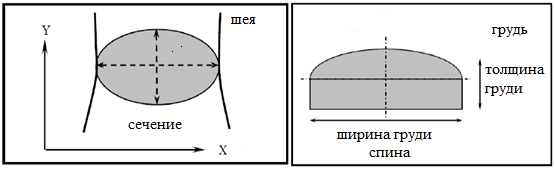
\includegraphics [width=0.8\linewidth] {images/h2.png}
\begin{center}
\caption{Примеры расчетов для обхвата шеи и груди.} \label{img2}
\end{center}
\end{figure}
\textit{1.5 Экспериментальное оценивание точности численного метода извлечения антропометрических признаков (п.2.3).} Оценка точности извлеченных признаков проведена использует анализ относительной среднеквадратической ошибки:
\begin{equation}\label{eq26}
\varepsilon_{rel}=\left\{\frac{\sum^{12}_{j=1}\left(\widetilde{z}_j - z_j\right)^2}{\sum^{12}_{j=1}z_j^2}\right\}^{1/2} = \frac{\left\|\widetilde{z} -z\right\|_2}{\left\|z\right\|_2},
\end{equation}
где $z_j$ -- результат измерений, рассчитанных вручную;
$\widetilde{z_j}$ -- результат измерений с помощью разработанного приложения. Использовалась база из 100 тестовых наборов изображений людей различного пола и телосложения. Кроме того, проведен подробный анализ ошибок измерений $\varepsilon = \left|\widetilde{z_j} - z_j\right|$ (см. рис. \ref{img16}а), при этом в первом случае использованы 24 опорных точек, а во втором - 28 точек. Экспериментально установлено, что  распределение случайной составляющей погрешности измерений (рис. \ref{img16}б) подчинено нормальному закону. В этом разделе также экспериментально установлена линейная сходимость предложенного численного метода на основе анализа апостериорной оценки погрешности при увеличении разрешения исходных изображений.
\begin{figure}[ht!]
\centering
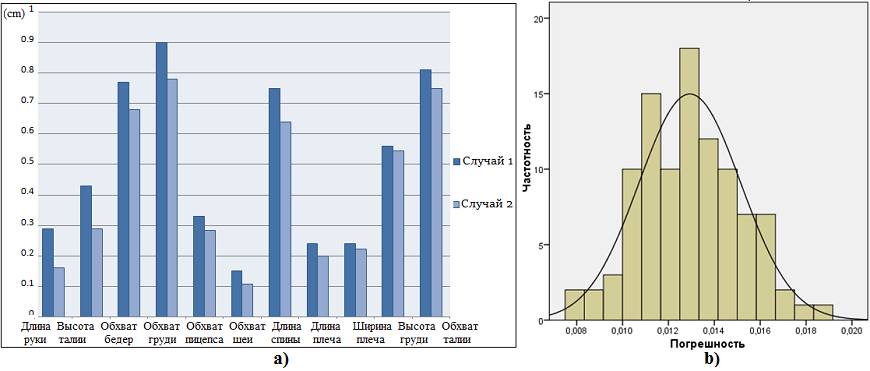
\includegraphics [width=0.96\linewidth] {images/h16.png}
\begin{center}
\caption{а) Погрешность $\varepsilon$. б) закон распределения погрешности измерений (сл. 2) по формуле (\ref{eq26}).} \label{img16}
\end{center}
\end{figure}

\textbf{2. Математическое моделирование типов телосложения.} Для построения 3D моделей экспериментальным путем было выявлено пять характеристических типов телосложения, по которым проводилась классификация. Каждый тип телосложения в свою очередь позволил строить 5 моделей. Кратко изложим адаптированную математическую модель для классификации антропометрических данных с помощью алгоритма случайного леса (Random Forest) (L. Breiman 2001). Пусть задан набор объектов $D=\left\{d_i|i=1, ..., N\right\}$, $X=\left\{x_i|i=1, ..., 12\right\}$ - набор антропометрических вектор-признаков и $Y=\left\{y_i|i=1, ..., 5\right\}$ - набор меток классов. Векторы антропометрических признаков $\left\{X_i\right\}^N_{i=1}$, в том числе каждый вектор имеет структуру $x_k=\left(x_{k1}, ..., x_{kd}\right)$. Модель обучения и тестирования использована для классификации объектов по меткам $Y$. Для оценки критерия качества построения решающих деревьев используется индекс Джини:
\begin{equation}\label{eq27}
Gini=N_L\sum^k_{i=1} p_{kL} \left(1-p_{kL}\right) + N_R\sum^k_{i=1} p_{kR} \left(1-p_{kR}\right),
\end{equation}
где $p_{kL}$ -- доля класса $K$ в левом узле ($N_L$), $p_{kR}$ -- доля класса $K$ в правом узле ($N_R$).
Предлагается алгоритм оценки и поиска набора признаков из исходного набора признаков. Алгоритм случайного леса состоит из двух основных этапа: обучение и тестирование. Процесс обучения осуществляется следующим образом:

\begin{itemize}
	\item взять из $D$ $n$ случайных объектов с повторениями (bootstrap sample) - $D_i$;
	\item построить для $D_i$ дерево, используя алгоритм <<дерево классификации и регрессии>> (CART) для построения решающего дерева. Причем для каждой вершины признак выбирается из $m$ случайно выбранных ($m$ - параметр, $1\leq m\leq p$);
	\item дерево строится до конца, без отсечения ветвей;
	\item повторить предыдущие шаги $B$ раз.
\end{itemize}
В итоге строится $B$ деревьев. Для проверки новых наборов антропометрических данных используются модели обучения.

\textbf{3. Задача построения антропометрических моделей.} В этом разделе представлен подход к реконструкции 3D-
\begin{figure}[ht!]
\centering
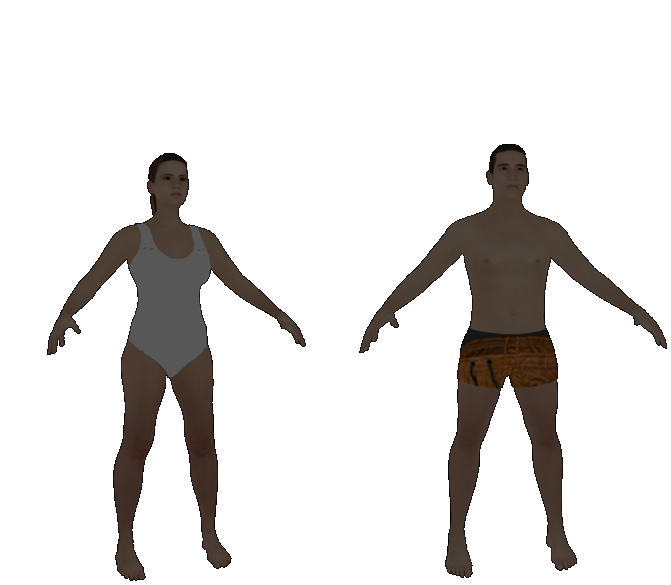
\includegraphics [width=0.6\linewidth] {images/h22.png}
\begin{center}
%\captionsetup{justification=justified, labelsep=period}
\caption{Примеры построенных моделей.} \label{img17}
\end{center}
\end{figure}
модели человека на основе антропометрических признаков, которые были предварительно извлечены и классифицированы. Использован набор данных антропометрических признаков для построения 3D-моделей телосложения.

Процесс построения антропометрических моделей включает следующие шаги:

\textbf{Шаг 1}: описание текстурных характеристик человеческого тела, а также текстуры одежды;

\textbf{Шаг 2}: разработка моделей частей человеческого тела (голова, туловище, руки, ноги) с использованием ранее полученных антропометрических признаков;

\textbf{Шаг 3}: построение текстурированной модели человеческого тела;

\textbf{Шаг 4}: экспорт модели человеческого тела в два файла: первый файл (*.mtl) описывает текстуры модели, второй файл (*.obj) содержает информацию каждой модели. На рис. \ref{img17} представлены примеры построения антропометрических моделей.

В \textbf {третьей главе} описывается проектирование системы компьютерного зрения в антропометрии для практических применений: моделирование одежды и фитнес-приложение. \mrk{Система проектируется с помощью аналитических методов объектно-ориентированного UML (рис. \ref{img35}). Программа описывается диаграммами: диаграмма прецедентов, диаграмма классов, диаграмма последовательности. Классы подробно анализируются с указанием задач каждого компонента в программе. Доказывается целесообразность проектирования приложений компьютерного зрения в антропометрии\cEA{Это здесь никого не интересует, важно как удалось алгоритмы в программы оформить.}.}
\begin{figure}[ht!]
\centering
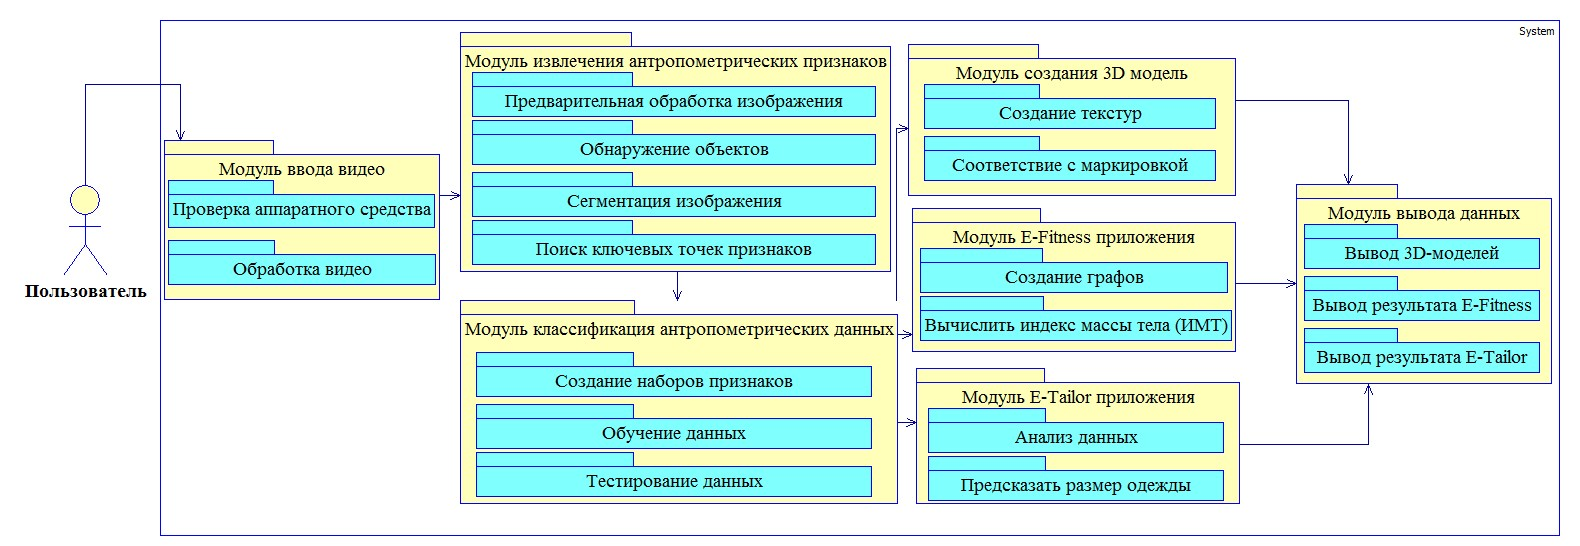
\includegraphics [width=0.95\linewidth]{images/h35.png}
\begin{center}
%\captionsetup{justification=justified, labelsep=period}
\caption{Структура ПО.} \label{img35}
\end{center}
\end{figure}

Проведен анализ практических результатов экспериментов извлечения антропометрических признаков. Выполнено сравнение результатов предложенных алгоритмов с другими алгоритмами по точности. Установлено преимущество синтеза алгоритма\cEA{Критерий? и что за синтез алгоритма?} на основе метода разреза на графах и итеративного алгоритма ближайших точек. И наконец, выполнено сравнение результатов классификации между алгоритмом случайного леса и алгоритмом Boosting, работающими с видео.

В \textbf{четвертой главе} дано описание среды разработки приложения Android, библиотек поддержки алгоритмов компьютерного зрения OpenCV\footnote{OpenCV - Open source computer vision [Electronic resource] // [http://opencv.org/] -- [S. l. : s. n.]. -- Дата доступа: 2017.}, поддержки построения 3D-моделей человеческого тела MakeHuman\footnote{MakeHuman library [Electronic resource] // [http://www.makehuman.org]. -- USA: [s. n.]. -- Дата доступа: 2017.} и библиотеки поддержки 3D для Android – Min3D\footnote{Softpedia. Min3D library [Electronic resource] // [https://code.google.com/p/min3d]. -- USA: [s. n.]. -- Дата доступа: 2017.}. Изложены инструкции для пользователей разработанных приложений\cEA{Это зачем? тут писать.}. Приведена архитектура мобильного приложения для моделирования одежды (E-Tailor). Главные функции приложения включают: автоматизацию извлечения антропометрических признаков и классификацию размеров одежды. Изложены этапы разработки приложения для фитнеса (E-Fitness). Главные функции разработанного приложения включают: автоматизацию извлечения антропометрических признаков, построение 3D-моделей человеческого тела, анализ и сравнение признаков телосложений, а также расчет индекса массы тела (ИМТ). Приложения разработаны на языке Java под ОС Android для смартфонов. Программные модули имеют простой, удобный и интуитивно понятный интерфейс\cEA{Выходит проблем с реализацией не было никаких? На каком этапе повышаем производительность, боремся с шумом, повышаем точность... Вероятно на этапах матмодели и численных методов.}.

\textbf{
\begin{center}
ОСНОВНЫЕ РЕЗУЛЬТАТЫ ДИССЕРТАЦИОННОЙ РАБОТЫ, ВЫНОСИМЫЕ НА ЗАЩИТУ
\end{center}
}

\begin{enumerate}
	\item[1)] Разработаны алгоритмы компьютерного зрения для извлечения антропометрических признаков, основанные на комбинации алгоритма сегментации изображений на основе метода разрезов на графах и итеративного алгоритма ближайших точек;
	\item[2)] Предложена модель и разработан и апробированы алгоритм классификации антропометрических данных методом случайного леса (Random Forest) для приложения, которое классифицирует объекты на основе антропометрических признаков;
	\item[3)] Разработаны алгоритмы и методы компьютерного зрения к задаче антропометрии на изображениях и видео с наличием шума и в режиме, близком к реальному времени\cEA{Результат пересекается с результатами 1 и 2. Надо четко выделить, что именно за антропометрия, на каком этапе (мерим части тела, например). Еще как-то охарактеризовать результат. См. п.1 и п.2. Там сказано на основе чего созданы алгоритмы - метод разреза..., случайный лес...};
	\item[4)] Построены антропометрические модели человеческого тела на основе результатов извлечения антропометрических признаков\cEA{Это примеры? или методика построения 3д-модели по результатам измерений разработана?};
	\item[5)] Разработанные алгоритмы и методы реализованы в виде двух приложений для смартфонов на ОС Андроид: приложение «E-Tailor» для моделирования одежды и приложение «E-Fitness» для фитнес-тестирования.
\end{enumerate}
\textbf{
\begin{center}
СПИСОК ОСНОВНЫХ РАБОТА ПО ТЕМЕ ДИССЕРТАЦИИ
\end{center}
}

\textbf{Издания, входящие в Перечень ВАК РФ:}

\begin{enumerate}
	\item Нгуен~Т.Л. Об автоматизации извлечения и классификации антропометрических признаков / Нгуен Т.Л., Нгуен Т.Х. // Вестник ИРНИТУ: №~4. 2015. -С. 17-23.
	\item  Nguyen~T.L. Studies of Anthropometrical Features using Machine Learning Approach / Nguyen T.L., Nguyen T.H., A. Zhukov // CEUR Workshop Proceedings. 2015, -V. 1452, -P. 96-105.
	\item Нгуен~Т.Л. О распознавании и классификации дефектов дорожного покрытия на основе изображений / Нгуен Т.Л., Нгуен Т.Х. // Вестник ИРНИТУ: №~10. 2016. -С. 111-118.
	\item Nguyen~T.L. Automatic Anthropometric System Development Using Machine Learning / Nguyen T. L., Nguyen T.H. // BRAIN. Broad Research in Artificial Intelligence and Neuroscience. 2016, -V. 7, -P. 5-15.\\
	\textbf{Издания, включенные в РИНЦ:}
	\item Nguyen T.H. A Robust Approach for Defects Road Pavement Detection and Classification/ Nguyen T. L., Nguyen T.H., D. N. Sidorov // Journal of Computational and Engineering Mathematics: 2016,-V. 3.-No. 3. -P. 40-52.\\
	\textbf{Свидетельства о государственной регистрации программы для ЭВМ:}
	\item  Сидоров Д.Н. Программа бесконтактной антропометрии для смартфонов на операционной системе Андроид // Сидоров Д.Н., Нгуен Т.Л., Нгуен Т.Х. // Свидетельство о гос. регистрации программы для ЭВМ. № 2016611475, от 03 февраля 2016 г. М.: Федеральная служба по интеллектуальной собственности. 2016.
	\item  Сидоров Д.Н. Программа автоматического обнаружения и классификации дефектов дорожного покрытия // Сидоров Д.Н.,  Нгуен Т.Х., Нгуен Т.Л. // Свидетельство о гос. регистрации программы для ЭВМ. № 2016619386, от 18 августа  2016 г. М.: Федеральная служба по интеллектуальной собственности. 2016.\\
\textbf{Прочие издания:}
\item  Нгуен Т.Л. Автоматизация антропометрических измерений и извлечение признаков из 2D-изображений / Нгуен Т.Л., Нгуен Т.Х. // Байкальская международная школа-семинар <<методы оптимизации и их приложения>>. О. Ольхон, Иркутск 2014г. -С. 153.
\item Нгуен Т.Л. Построение программы для обнаружения контуров человека в изображении с помощью методов математической морфологии / Нгуен Т.Л., Нгуен Т.Х. // Материалы всероссийской молодежной научно-практической конференции <<Винеровские чтения 2014>>. Иркутск: Изд-во Иркутск, 2014. -С 10.
\item Нгуен Т.Л. Классификация и кластерный анализ антропометрических признаков / Нгуен Т.Л.// Материалы всероссийской молодежной научно-практической конференции <<Винеровские чтения 2015>>. Иркутск: Изд-во Иркутск, 2015. -С.8.
\item Нгуен Т.Л. Методы математической морфологии в цифровой обработке изображений / Нгуен Т.Л., Нгуен Т.Х. // Труды XIX Байкальской Всероссийской конференции <<информационные и математические технологии в науке и управлении>>. Иркутск: ИСЭМ СО РАН, 2014. -С. 75-81.
\item Нгуен Т.Л. Анализ антропометрических признаков с использованием методов машинного обучения / Нгуен Т.Л., Нгуен Т.Х. // Междисцплинарные исследования в области математического моделирования и информатики . Ульяновск: Изд-во SIMJET, января 2015г.-С.204-210.
\item Nguyen T.L. On Road Defects Detection and Classification / Nguyen T.L., Nguyen T.H., A. Zhukov // Supplementary Proceedings of the 5th International Conference on Analysis of Images, Social Networks and Texts (AIST 2016). CEUR Workshop Proceedings, 2016,-V. 1710, -P. 266- 278.
\end{enumerate}

%%% Local Variables:
%%% mode: latex
%%% TeX-master: "../synopsis"
%%% End:
